% in Anlehnung an https://github.com/derdanu/akad-vorlage
% Autor: Lukas Lück
%-------------------------------------------
% Vorgaben Assignment aus Studienheft SQL301
%-------------------------------------------
% Umfang: 8 - 10 Seiten (inkl. Abbildungen und Tabellen, ohne Deckblatt, Gliederung und Literaturverzeichnis, Eidesstattliche Erklaerung)
% Zeilenabstand: 1,5, Tabellen 1,0 
% Schriftart: frei
% Schriftgrad: 11 oder 12 pt
% Tabellen auch 10pt
% Silbentrennung ok, auf "Missratene" Trennung achten!
% Variablen, physikalische Groessen und Funktionszeichen werden kursiv gedruckt.
% Ränder: links: 4,5 cm, rechts 2,0 cm, oben und unten jeweils 3,0 cm
% Deckblatt: (Name, Adresse, AKAD-E-Mail-Adresse, Immatrikulationsnummer, Modulbezeichnung, Thema, Abgabedatum, Dozent)

% Reihenfolge (siehe SQL301, S. 71):
% Titelblatt, ohne Nummerierung
% Inhaltsverzeichnis (ohne Nummerierung) -> Abbildungsverzeichnis (Nummerierung in Römisch, beginnend mit "III")-> Tabellenverzeichnis -> Abk.-Verzeichniss
% Textteil, Nummerierung in arabisch, beginnen mit "1"
% Anhang -> Literaturverzeichnis, Nummerierung in Römisch, folgend auf Römische Nummerierung von Verzeichnissen

\documentclass[listof=totoc, bibliography=totoc, a4paper, 12pt, numbers=noenddot]{scrartcl}
\usepackage[ngerman]{babel}
\usepackage{epsfig}
\usepackage{times}
\usepackage{tabto}
\usepackage{wrapfig}
\usepackage{multirow}
\usepackage[onehalfspacing]{setspace}
\usepackage{listings}
\usepackage{mathptmx}
\usepackage{geometry}
\usepackage{helvet}
\usepackage{courier}
\usepackage{setspace}
\usepackage{textcomp}
\usepackage[T1]{fontenc}
\usepackage[utf8]{inputenc}
\usepackage{fancyhdr}
\fancyheadoffset{0pt}% <- added
\usepackage{lastpage}
\usepackage{etoolbox}
\usepackage{hyphenat} %Silbentrennung für einzelne Wörter verhindern mit \nohyphens{text}
\usepackage{float} % Notwendig fuer figure[h]
\usepackage[printonlyused]{acronym}
\usepackage{multicol} % für zweispaltiges Deckblatt
\usepackage{microtype}%"entspanntere" Umbrüche
% Pakete für Literatur + zitieren, authoryear-ibid
\usepackage[backend=biber, style=authoryear-ibid, autocite=footnote, maxnames=4, ibidpage=true, dashed=false]{biblatex} %maxnames: Maximale anzieg im Verzeichnis, danach u.a.; dashed: bei gleichen Autoren würde bei true beim zweiten Eintrag ein"-" erschienen anstelle des Autors
\usepackage{csquotes}
\usepackage{xpatch}
\addbibresource{Literatur/literatur.bib}

\usepackage[table,xcdraw]{xcolor}
\usepackage{longtable}
\usepackage{lscape}
\usepackage[font=normalsize]{caption}
\usepackage{graphicx}
\usepackage{vcell}
\usepackage{colortbl}
\usepackage{hhline}
%Bei Tabellen mit anderer Schriftgröße wird Index in normaler Schriftgröße angezeigt
%\usepackage{pgfplotstable} %Tabellen transponieren

%\usepackage{pdfpages}%Einbinden vpn pdf-Dateien
% Allgemeine Definitionen

% Assignmentbezeichnungen
%-----------------------------------------------------------------------------------
\newcommand*{\assi}{Assignment REG23-AS-002}
% Titel
\newcommand*{\titel}{Steuerungs- und Regelungstechnik} 
% Betreff
\newcommand*{\betreff}{Thema \glqq Bohreinrichtung\grqq{} } 
% Modul
\newcommand*{\modul}{REG23}
% Betreuer
\newcommand*{\dozent}{Heimerdinger} 
% Vor- und Nachname
\newcommand*{\name}{Papa Schlumpf}
% Straße und Hausnummer
\newcommand*{\strasse}{Am Pilz 01} 
% Plz und Ort
\newcommand*{\plzort}{1234 Schlumpfhausen} 
% Immatrikulationsnummer
\newcommand*{\immanr}{123456789}
% Studiengang
\newcommand{\stud}{Mechatronik - Bachelor of \tabto{40mm}Engineering (B. Eng.)}
%-----------------------------------------------------------------------------------

% URL in gleicher Schriftart wie Rest
\urlstyle{same}
% Email mit Verlinkung
\newcommand*{\email}{\href{mailto:hier_könnte_deine E-Mail_stehen@test.de}{hier_könnte_deine_Email_stehen@x.de}} 

% Formatierungen für das Literaturverzeichnis
%--------------------------------------------
% Doppelpunkt und Leerzeichen nach Autor
\renewcommand*{\labelnamepunct}{\addcolon\addspace} 
% Punkt am Ende entfernen
\renewcommand*{\finentrypunct}{\addspace}
% Komma zwischen einzelnen Einträgen
\renewcommand*{\newunitpunct}{\addcomma\addspace}
% Punkt am Ende von Zitaten entfernen
\renewcommand*{\bibfootnotewrapper}[1]{\bibsentence#1\addspace}
% Zeilenabstand zwischen einzelnen Einträgen
\setlength{\bibitemsep}{0.5\baselineskip}
\usepackage[
pdftitle={\titel},
pdfsubject={Assignment zum Modul AUT21},
pdfauthor={\name},
pdfkeywords={Akad, Assignment, AUT21, Piezo-Sensoren, Wirbelfrequenzzähler},
pdfborder={0 0 0},  % Links nicht sichtbar im pdf
colorlinks = false,
pdfpagelabels,
pdfstartview = FitH,
bookmarksopen = true,
bookmarksnumbered = true,
linkcolor = black,
plainpages = false,
hypertexnames = false,
urlcolor = black,
citecolor = black] {hyperref}

\usepackage{url}

%URl-Definition für URL mit "%" im Link
\urldef\lmDat\url{https://www.ti.com/lit/ds/symlink/lm35.pdf?ts=1682065674820&ref_url=https%253A%252F%252Fwww.ti.com%252Fproduct%252FLM35}


\newcounter{savepage} % Zähler für Seitenzahl, für später ab Römischer Nummerierung
%--------------------------------------------------------------------------------------------------------------------------------
%                                       Dokument begin
%--------------------------------------------------------------------------------------------------------------------------------
\begin{document}

% Deckblatt
% Festlegung der Seitenränder
\newgeometry{left=20mm, right=20mm, top=30mm, bottom=30mm}
\thispagestyle{empty}
{
    % Zentrieren der gesamten Seite
    \centering
    
    % Abstand von oben
    \vspace*{3cm}
    % Titel der Arbeit
    {\Huge\textbf{\docType}}\\
    \vspace*{2cm}
    {\Huge{\docTitle}}\\
    \vspace*{1cm}
    {\Large{\betreff}}\\
    \vspace*{2cm}

    \begin{table}[H]
        \centering
        \begin{tabular}{ll|ll}
            Name, Vorname:       & \name                        & Studiengang: & \studiFieldOne  \\
            Immatrikualtionsnr.: & \immanr                      &              & \studiFieldTwo  \\
            Adresse:             & \strasse                     & Modul        & \modul          \\
                                 & \plzort                      & Abgabe am:   & \finalDate      \\
            E-Mail               & \href{mailto:\mail}{\mail}   & Dozent       & \dozent                  
        \end{tabular}
    \end{table}
    
    % Abstand von unten
    \vfill
    
    % Institution
    
\includegraphics[scale=0.35]{Ressources/Bilder/akad_logo.png}\par
}







\newgeometry{left=45mm, right=20mm, top=30mm, bottom=30mm}

\begin{spacing}{1.0} % Verzeichnisse werden mit einzeiligem Abstand gesetzt

% Inhaltsverzeichnis ohne Nummerierung
\pagestyle{fancy}
\fancyhead{}
\renewcommand{\headrulewidth}{1pt}
\fancyhead{}
\fancyfoot{}
\pagenumbering{Roman}
\setcounter{page}{2}
% Inhaltsverzeichnis
\pdfbookmark{\contentsname}{toc}
\tableofcontents 
\newpage

% ab hier Nummerierung oben in Römisch, beginnend mit 3
\pagestyle{fancy}
\fancyhead{}
\renewcommand{\headrulewidth}{1pt}
\fancyhead[R]{\thepage}
\fancyfoot{}
\pagenumbering{Roman}
\setcounter{page}{3}

% bei Nichtbedarf entsprechende Zeile Auskommentieren:

% Abbildungsverzeichnis, 
\listoffigures 
\newpage

% Tabellenverzeichnis
\listoftables 
\newpage

% Abkürzungsverzeichnis
%\section*{Abkürzungsverzeichnis}
\addcontentsline{toc}{section}{Abkürzungsverzeichnis} 
\begin{acronym}
        \acro{SPS}{speicherprogrammierbare Steuerung}
\end{acronym}
%\newpage

% Formelverzeichnis
%\listof{Formel}{Formelübersicht}
\setcounter{savepage}{\value{page}} %speichert Seitenzahl für spätere folgende Römische Nummerierung
\end{spacing} 


% ab hier Nummerierung oben in arabisch, beginngend mit 1
\pagestyle{fancy}
\fancyhead{}
\renewcommand{\headrulewidth}{1pt}
\fancyhead[R]{\thepage}
\fancyfoot{}
\pagenumbering{arabic}

\begin{spacing}{1.5} % Zeilenabstand: 1,5 fuer den Textteil
%-------------------------------------------------------------------------------------------------------------------
%                     Ab hier der eigentliche Textteil
%-------------------------------------------------------------------------------------------------------------------
% Einleitung
\sloppy%Leerräume dürfen gedehnt werden
\pdfbookmark{Kapitel}{kapitel}
\section{Einleitung}

\section{Hinführung}
Das ist ein Tes kjbsdkjafnadpk alsdh lk a. Das ist eine Abkürzung: \ac{api}.\autocite[vgl.][S. 20]{book:SimulationMechatronischerSysteme}
    
        
\subsection{Problemstellung}
    
    
\subsection{Ziel der Arbeit}
    
    
\subsection{Aufbau der Arbeit}
    


% Grundlagen
\section{Physikalische Grundlagen}
\subsection{Der piezoelektrische Effekt}
Das Wort \textit{\glqq piezo\grqq{}} stammt vom griechischen Wort \textit{\glqq pi\'{e}zein = drücken\grqq{}} ab. Erstmals wurde der piezoelektrische Effekt 1880 durch die Brüder Pierre und Jacques Curie entdeckt.\autocites[vgl.][]{duden01}[vgl.][]{Curie}\\
Wird ein Kristallgitter durch äußeren Druck verformt, entsteht an den Oberflächen eine elektrische Ladung \textit{Q}. Dies führt zu einer messbaren Spannung. Die erzeugte Ladung \textit{Q} ist direkt proportional  zum Druck \textit{p}, der einwirkenden Fläche \textit{A} sowie dem stoffabhängigen Piezomodul \textit{k}:
\begin{eqnarray}
    Q=k \cdot A \cdot p
\end{eqnarray}
In Abbildung \ref{fig:piezoeffekt} ist der Piezoeffekt am Kristallgitter von $SiO_2$ dargestellt. Abhängig von der Druckachse zur polaren Achse des Kristalls unterscheidet man zwischen dem longitudinalen (\ref{fig:piezoeffekt}b) oder dem transversalen Effekt (\ref{fig:piezoeffekt}c). Vorallem letzterer findet in der Praxis Anwendung. Piezoelektrische Sensoren weisen aufgrund ihrer geringen Temperaturabhängigkeit hohe Messgenauigkeiten auf. Hauptsächlich werden diese Sensoren in dynamischen Messungen mit hohen Messfrequenzen eingesetzt. \autocites[vgl.][260 \psqq]{Sensoren}[vgl.][273 \psq]{Physik}

\begin{figure}[H]
   \centering
    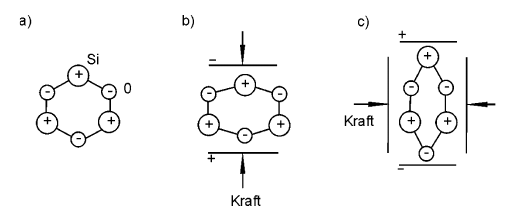
\includegraphics[scale=0.6]{Bilder/Piezoeffekt.png}
    \caption[Darstellung des Piezoeffekts]{Piezoeffekt am Kristallgitter von $SiO_2$ \footnotemark}
    \label{fig:piezoeffekt}
\end{figure}
\footnotetext{\cite{Physik}}
Die Umkehrung des piezoelektrischen Effekts, auch \textit{Elektrostriktion} genannt, ist ebenso möglich. Hier wird eine elektrische Feldstärke \textit{E} an einen geeigneten Kristall angelegt. Dies führt zu einer Längenänderung \textit{$\epsilon$}. \autocite[vgl.][274]{Physik} Die bekannteste Anwendung dieses Effekts ist der Injektor zum Einspritzen von Dieselkraftstoffen. Hierbei sind mehrere Piezoelemente in Reihe als sogenannte Stacks geschalten und bewirken bei Anlegung einer Spannung den Nadelhub der Einspritzdüse. Der piezoelektrische Effekt lässt sich somit als Sensor und Aktor nutzbar machen. 
%------------------------------------------------------------------------------
%------------------------------------------------------------------------------
%------------------------------------------------------------------------------
\subsection{Grundlagen der Strömungsmechanik}
In der Strömungsmechanik, vor allem in Rohrleitungen, unterscheidet man zwischen laminaren (geschichteten) und turbulenten (ungeordneten) Strömungen. Bei einer laminaren Strömung fließen die Fluidteilchen in Hauptstromrichtung ohne Querbewegungen. In turbulenten Strömungen werden die Fluidteilchen aufgrund von Reibungskräften zusätzlich quer zur Hauptströmung abgelenkt. Dadurch entstehen Wirbel. Für die Beschreibung der Strömung wurde die dimensionslose Reynolds-Zahl \textit{Re} eingeführt. Sie beschreibt das Verhältnis der kinetischen Energie und der Reibungsenergie:
\begin{eqnarray} \label{for:Re}
    Re &=&\frac{\rho \cdot L \cdot u}{\eta}\\
    mit: \quad \rho &=& Dichte \nonumber \\
    L &=& L\ddot{a}nge~ des ~umstr\ddot{o}mten ~ K\ddot{o}rpers \nonumber \\
    u &=& Str\ddot{o}mungsgeschwindigkeit \nonumber \\
    \eta &=& Z\ddot{a}higkeit ~ des ~ Mediums  \nonumber
\end{eqnarray}
In Rohrleitungen liegt für kleine Reynolds-Zahlen von $Re = 100$ bis $Re_{krit} = 2320$ eine laminare Strömung vor. Für $Re > 2320 $ treten mit steigender $Re$ immer stärkere Wirbel auf und die Strömung wird turbulent. Für umströmte Profilkörper variiert die kritische Reynolds-Zahl $Re_{krit}$. \autocites[vgl.][63]{Physik}[vgl.][342]{Böge} \\
Wird ein Körper umströmt, so entstehen an seinen Ablösepunkten Wirbelablösungen. Ab einer Reynolds-Zahl von $Re \approx 40$ bis $Re = 2 \cdot 10^5$ treten die Wirbel periodisch auf. Dieses Phänomen wird nach seinem Entdecker Theodor von K\'{a}rm\'{a}n (1881-1963) auch als K\'{a}rm\'{a}n`sche Wirbelstraße bezeichnet (siehe Abbildung \ref{fig:wirbelstrasse}, Seite \pageref{fig:wirbelstrasse}). \autocite[vgl.][441 \psq]{Surek}

\begin{figure}[H]
   \centering
    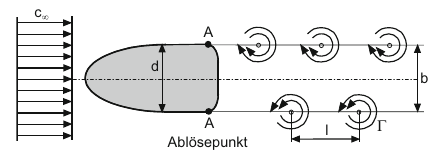
\includegraphics[scale=0.75]{Bilder/Wirbelstrasse.png}
    \caption[K\'{a}rm\'{a}n`sche Wirbelstraße]{K\'{a}rm\'{a}n`sche Wirbelstraße an einem umströmten Körper \footnotemark}
    \label{fig:wirbelstrasse}
\end{figure}
\footnotetext{\cite[][442]{Surek}}
Eine weitere dimensionslose Zahl ist die Strouhal-Zahl. Sie ist als Verhältnis der lokalen zur konvektiven Beschleunigung definiert:\autocite[vgl.][352]{Böge}
\begin{eqnarray}\label{for:Sr}
    Sr&=&\frac{f \cdot d}{u}\\
    mit: \quad f &=& Abl\ddot{o}sefrequnez \land d = K\ddot{o}rperdicke \land \nonumber \\
    u &=& Str\ddot{o}mungsgeschwindigkeit \nonumber
\end{eqnarray}
In Abbildung \ref{fig:re_sr} ist die Abhängigkeit der Strouhal-Zahl $Sr$ von der Reynolds-Zahl $Re$ dargestellt. Im Bereich von $Re \approx 100$ bis $Re \approx 2 \cdot 10^5$ ist die Strouhal-Zahl $Sr \approx 0,2$. Dieser Umstand wird sich bei Wirbelstromzählern zunutze gemacht. Mithilfe der gemessenen Ablösefrequenz $f$ und der bekannten Staukörperdicke lässt sich die Anströmgeschwindigkeit $u$ ermitteln. \autocite[vgl.][442]{Surek}

\begin{figure}[H]
    \centering
    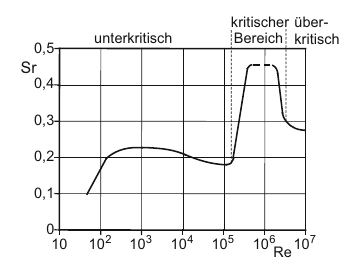
\includegraphics[scale=0.75]{Bilder/Re_Sr.png}
    \caption[Strouhal-Zahl in Abhängigkeit der Reynolds-Zahl]{Strouhal-Zahl Sr in Abhängigkeit der Reynolds-Zahl Re\footnotemark}
    \label{fig:re_sr}
\end{figure}
\footnotetext{\cite[][442]{Surek}}
%Mit den bisher vorgestellten physikalischen Grundlagen der Strömungsmechanik lässt sich im Folgenden die Funktionsweise eines Wirbelstromzählers beschreiben.
%------------------------------------------------------------------------------
%------------------------------------------------------------------------------
%------------------------------------------------------------------------------





% Hauppteil
\section{Wirbelfrequenzzähler}
\subsection{Aufbau und Funktionsweise eines Wirbelfrequenzzählers}
In Abbildung \ref{fig:wirbelzaehler} ist der typische Aufbau eines Wirbelfrequenzzählers, auch Wirbeldurchflussmesser genannt, dargestellt. Im Wesentlichen besteht dieser aus einem Messrohr(4), in dem ein Staukörper(1) mit bestimmter Geometrie(5) eingelassen ist. Hinter diesem ist ein Wirbeldruckabnehmer (2) verbaut. Das erzeugte Signal wird von einer Auswertelektronik verarbeitet und dem Anwender ausgegeben.\autocite[vgl.][803\psqq]{Sensortechnik}
\begin{figure}[H]
   \centering
    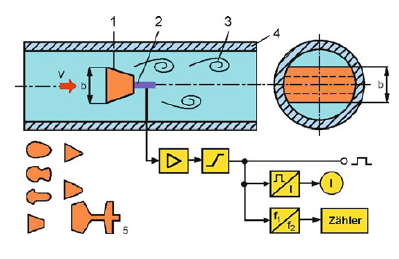
\includegraphics[scale=0.75]{Bilder/Wirbelzaehler.png}
    \caption[Aufbau eines Wirbeldurchflussmessers]{Aufbau eines Wirbeldurchflussmessers\footnotemark}
    \label{fig:wirbelzaehler}
\end{figure}
\footnotetext{\cite[][291]{Sensoren}}
Das Messprinzip beruht auf der K\'{a}rm\'{a}n`schen Wirbelstraße. Durch den Staukörper entstehen bei strömenden Medien sich periodisch abwechselnde Wirbel. Diese erzeugen hinter der Staugeometrie einen Unterdruck, der ebenso periodisch variiert. Die Druckschwankung bringt den Wirbeldruckabnehmer in Schwingung. Mithilfe eines Sensorelements wird die Frequenz $f$ der Schwingung in ein elektrisch auswertbares Signal umgewandelt. Dies kann mechanisch, akustisch oder optisch erfolgen.\autocite[vgl.][S. 803]{Sensortechnik}\\
Die mathematische Ermittlung der Strömungsgeschwindigkeit $u$ beruht auf der Proportionalität zur Ablösefrequenz $f$: 
\begin{eqnarray}\label{for:f}
    f &=& K_1 \cdot u \\
    mit: \quad K_1 &=& Proportionalit\ddot{a}tsfaktor \nonumber
\end{eqnarray}
Desweiteren gilt für den Volumenstrom $Q_v$ folgende Abhängigkeit:
\begin{eqnarray}
    Q_v &=& u \cdot A \\
    mit: \quad A &=& Messrohrquerschnitt \nonumber
\end{eqnarray}
Der Messrohrquerschnitt $A$ ist bei dem jeweiligen Wirbelfrequenzzähler konstant, sodass sich für den Kalibrierfaktor $K$ eines Wirbelzählers folgender Zusammenhang besteht:
\begin{eqnarray}
    f &=& K \cdot Q_v
\end{eqnarray}
Somit kann der Volumenstrom direkt aus der gemessenen Ablösefrequenz $f$ und des Kalibrierfaktors $K$ berechnet werden. Setzt man Formel (\ref{for:f}) in die Formel (\ref{for:Sr}), Seite \pageref{for:Sr} ein, erhält man für den Proportionalitätsfaktor $K_1$:
\begin{eqnarray}
    S_r &=& K_1 \cdot d
\end{eqnarray}
Da die Strouhal-Zahl $Sr$ in einem bestimmten Bereich der Reynolds-Zahl $Re$ nahezu konstant ist, kann der Proportionalitätsfaktor $K_1$ und damit auch der Kalibrierfaktor $K$ bestimmt werden. In der Regel wird dieser jedoch nicht berechnet, sondern direkt vom Hersteller kalibriert.\autocite[vgl.][S. 806 \psq]{Sensortechnik}

\subsection{KROHNE OPTISWIRL 4200}
Der $OPTISWIRL \: 4200$ der Firma  $KROHNE$ arbeitet nach dem Prinzip der K\'{a}rm\'{a}n`schen Wirbelstraße. Die Sensoreinheit zur Erfassung der Wirbelfrequenz ist im Benutzerhandbuch nicht näher ausgeführt, jedoch sind im Kapitel \textit{\glqq Statusmeldungen und Diagnose-Informationen\grqq{}}, Seite 96 des Benutzerhandbuches unter der Ereignisgruppe \textit{\glqq Sensor\grqq{}} Fehlermeldungen beschrieben, die sich auf ein Piezoelement beziehen. Somit kann davon ausgegangen werden, dass die primäre Messgröße (Anzahl der abgelösten Wirbel) mithilfe eines Piezoelements erfasst wird. Die periodische Druckschwankung wirkt auf das Piezoelement und erzeugt ein periodisch schwankendes, elektrisches Potenzial, welches der Wirbelfrequenz entspricht. Als sekundäre Messgröße gibt der Hersteller zusätzlich den Betriebs-, Norm-, Volumen- und -Massedurchfluss an. Weiterhin kann die Temperatur und optional der Druck erfasst werden. Den $OPTISWIRL \: 4200$ gibt es in verschiedenen Ausführungen, die sich nach dem jeweiligen Einsatzzweck richten. \autocite[vgl.][96, 107 \psq]{Optiswirl}

\subsection{Endress+Hauser Prowirl 200}
Die Firma \textit{Endress+Hauser} stellt ebenso ein Wirbeldurchflussmessgerät her, welches das Prinzip der K\'{a}rm\'{a}n`schen Wirbelstraße nutzt. Die Wirbelfrequenz wird beim  $Proline \: Prowirl \: F \: 200$ mithilfe eines kapazitiven Sensors in ein elektrisch auswertbares Signal umgewandelt. Vereinfacht dargestellt, besteht dieser Sensor aus zwei parallel gegenüberliegenden Kondensatorplatten. Der Abstand zwischen den Kondensatorplatten kann durch äußere Einwirkungen variieren. Dadurch verändert sich die Kapazität des Kondensators, die messtechnisch erfasst und ausgewertet wird. Zusätzliche Messgrößen können wie beim $OPTISWIRL \: 4200$ ebenso erfasst werden. Als Alleinstellungsmerkmal bewirbt \textit{Endress+Hauser} den $Proline \: Prowirl \: F \: 200$ mit einer integrierten Nassdampferkennung. Die Kalibrierung des Proportionalitätsfaktors $K$ ist für nicht abrasive Medien auf \textit{\glqq Lebenszeit\grqq{}} angegeben, da der Sensor keinem Langzeit- oder Nullpunktdrift unterliegt. In abrasiven Medien kann sich jedoch die Geometrie des Staukörpers geringfügig ändern. Dies verändert den $K-Wert$, sodass eine Neukalibrierung nach bestimmten Zeitabständen erforderlich ist.\autocites[vgl.][476 \psq]{Sensortechnik}[vgl.][4 \psq]{Prowirl}

\subsection{Gegenüberstellung der beiden Messgeräte}
In Tabelle \ref{tab:uebersicht}, Seite \pageref{tab:uebersicht} sind die wichtigsten technischen Eigenschaften der beiden Hersteller gegenübergestellt. Als Nennweite wurde $DN25$  gewählt. Diese Kenngröße ist ein typisches Merkmal von Rohrleitungssystemen. Sie folgt der $DIN \: EN \: ISO \: 6708$ und stellt sicher, dass zueinander gehörende Bauteile bei Rohrleitungssystemen passgenau sind. Die Innendurchmesser sind annähernd gleich. Dadurch ist der Vergleich und die Leistungsbeurteilung der einzelnen Messgeräte möglich.\autocite[vgl.][399]{technischesZeichnen}\\
Die Einsatztemperatur ist für beide Geräte annähernd gleich. Trotzdem ist der $Prowirl \: F \: 200$ für höhere Messstofftemperaturen geeignet. Bei der Durchflussgeschwindigkeit weist der $OPTISWIRL$ ein kleineres Spektrum auf als das Konkurenzprodukt. Für geringere Durchflussgeschwindigkeiten von Gasen und Dämpfen ist der $Prowirl \: F \: 200$ aufgrund der minimalen Fließgeschwindigkeit von $0,7 \frac{m}{s}$ geeignet. Jedoch liegt die maximale Durchflussgeschwindigkeit beim $Prowirl \: F \: 200$ unter dem Wert des zweiten Produkts. Der maximale Messdruck sowie die Genauigkeit der ermittelten Messwerte ist bei beiden gleich. Die Versorgungsspannung kann beim $Prowirl \: F \: 200$ um $5V$ höher bei maximal $35V$ liegen. Beide Messgeräte unterstützen die gängigen Kommuniktationsschnittstellen für den Industriegebrauch, der $Prowirl \: F \: 200$ verfügt zusätzlich über eine von \textit{Endress+Hauser} entwickelte Serviceschnittstelle. Für den $OPTISWIRL \: 4200$ lässt sich dazu im Benutzerhandbuch keine Information finden.\autocites[vgl.][9 \psqq]{Prowirl}[vgl.][108 \psqq]{Optiswirl}
\input{Tabellen/gegenueberstellung}
Die Preise für die jeweiligen Wirbelfrequenzzähler sind öffentlich nicht einsehbar. Gebrauchte Geräte auf dem freien Markt lassen allerdings die Schlussfolgerung zu, dass das Messgerät der Firma \textit{Endress+Hauser} deutlich höher ausfällt, als das Modell des Konkurrenten. Welches Messgerät besser ist, lässt sich pauschal jedoch nicht feststellen, da der Einsatzzweck, das verwendete Medium und der Kostenrahmen in der Regel die entscheidenden Faktoren sind.\autocites[vgl.][]{KostenOptiswirl}[vgl.][]{KostenProwirl}

% Schluss
\section{Schlussbetrachtung}
\subsection{Zusammenfassung}
In diesem Assignment wurde die Anwendung von Piezo-Sensoren in der Prozessmesstechnik beschrieben. Dazu wurde zuerst der piezoelektrische Effekt dargestellt. Anschließend erfolgte eine Einführung in die Grundlagen der Strömungsmechanik. Besondere Beachtung fand dabei die Reynolds-Zahl, die K\'{a}rm\'{a}n`sche Wirbelstraße und die Strouhal-Zahl. Mit den erarbeiteten physikalischen Grundlagen konnte die Anwendung von Piezo-Sensoren in der Prozessmesstechnik anhand des Wirbelfrequenzzählers beschrieben werden. Dazu wurde im ersten Schritt der allgemeine Aufbau und die Funktionsweise dieses Messgerätes erarbeitet. Anschließend wurden Wirbelfrequenzmessgeräte der Hersteller $KROHNE$ und \textit{Endress+Hauser} als Beispiel näher beschrieben. Hierbei wurde bereits festgestellt, dass die Messgrößenerfassung nur bei der Firma $KROHNE$ auf einem Piezoelement beruht. Als Abschluss dieses Assignment wurden die beiden Messgeräte gegenübergestellt und markante technische Daten verglichen.
%-------------------------------------------------------------------------------------------------------------------
%-------------------------------------------------------------------------------------------------------------------
\subsection{Kritische Reflexion}
Bei der Literaturrecherche wurde bereits deutlich, dass es eine Vielzahl von physikalischen Prinzipien zur Durchflussmessung gibt. Genauso vielfältig sind auch die Sensoren zur Erfassung der Messgrößen. Dementsprechend müssten die physikalischen Grundlagen auf weitere Gesetzmäßigkeiten ausgeweitet werden. Beispielsweise wird bei dem $Prowirl \: F \: 200$ ein kapazitiver Sensor verwendet. Hier konnte aufgrund des Umfangs des Assignments nur auf Piezo-Sensoren eingegangen werden. Die technischen Eigenschaften der Wirbelfreuqenzzähler wurde nur sehr allgemein betrachtet. Heutige Messgeräte umfassen deutlich mehr Parameter. Mit Blick auf die Industrie 4.0 wird sich in Zukunft der Funktionsumfang von Messgeräten zusätzlich steigern. Auch hier würde eine detaillierte Beschreibung den Umfang des Assingments übersteigen. Abschließend kann festgehalten werden, dass die Ausarbeitung einen guten Einblick in die komplexe Thematik der Anwendung von Piezo-Sensoren in der Prozesstechnik gibt.
\end{spacing}

% ab hier Römisch, folgend auf Verzeichnisse
\pagenumbering{Roman}
\setcounter{page}{\value{savepage}}

% Anhang, bei Nichtbedarf auskommentieren
%\newgeometry{left=30mm, right=10mm, top=30mm, bottom=20mm}
%Original: \newgeometry{left=45mm, right=20mm, top=30mm, bottom=30mm, landscape}

\section*{Anhang}
\addcontentsline{toc}{section}{Anhang}
\renewcommand{\thesubsection}{\Alph{subsection}}
%Begin Anhang
\subsection{Shared-Memory-API} \label{anhang:sharedMemApi}


\begin{landscape}
\subsection{Fehleruntersuchung}\label{anhang:error_analysis}
    %\input{Tabellen/error_analysis}
\end{landscape}

                    

%[frame=leftline,  fontsize=\scriptsize, breaklines=true, linenos, ]

    






   


% Literaturverzeichnis
\pdfbookmark{Literaturverzeichnis}{literaturverzeichnis}
\printbibliography[notkeyword=Bilder, notkeyword=Teile, title=Literaturverzeichnis]
%\printbibliography[keyword=Bilder, heading=subbibliography, title={Bildernachweis}]
%\printbibliography[keyword=Teile, heading=subbibliography, title={Nachweis Teileliste}]

\end{document}
